\chapter{Condizioni di funzionamento normali: il regime permanente}
Nello studio del regime permanente, il sistema con trasmissione su rete è costituito da linee con trasformatori in partenza e in arrivo, generatori sincroni e carichi elettrici.

Il sistema si suppone trifase simmetrico, cioè costituito da componenti già intrinsecamente simmetrici (generatori sincroni, trasformatori e carichi) o resi tali mediante trasposizione ciclica dei conduttori di linea, in condizioni di funzionamento normale. Poiché in ogni sezione della rete le terne delle tensioni e delle correnti costituiscono sistemi simmetrici ed equilibrati di sequenza diretta, l'analisi può essere condotta considerando una sola delle tre fasi mediante il circuito monofase equivalente alla sequenza diretta. Determinate le grandezze relative alla fase di riferimento, le corrispondenti grandezze delle altre due fasi si ottengono moltiplicando per gli operatori complessi $\bar{\alpha} = e^{j\frac{2\pi}{3}}$ e $\bar{\alpha}^2 = e^{j\frac{4\pi}{3}}$, che introducono uno sfasamento reciproco pari a $120^\circ$.

\section{Modello per la linea di trasmissione}
Le costanti primarie consentono di attribuire a ciascuna fase una resistenza $r$, una conduttanza $g$, un'induttanza di servizio $L_s$ e una capacità di servizio $C_s$, disaccoppiando le tre fasi della linea. Tuttavia, tali grandezze sono uniformemente distribuite lungo l'intero sviluppo chilometrico del conduttore, per cui non risulta immediata l'individuazione di un circuito equivalente a costanti concentrate per la rappresentazione compatta in regime permanente.

\subsection{Equazioni dei telegrafisti e risoluzione analitica}
Si considera l'elemento infinitesimo di linea di lunghezza $dx$, compreso tra le ascisse generiche $x$ e $x + dx$, associato al circuito monofase equivalente a parametri distribuiti. Il conduttore di ritorno, denominato neutro, costituisce un conduttore fittizio a impedenza longitudinale nulla che fornisce la via di richiusura per le correnti e il riferimento per i potenziali.
\begin{figure}[H]
	\centering
	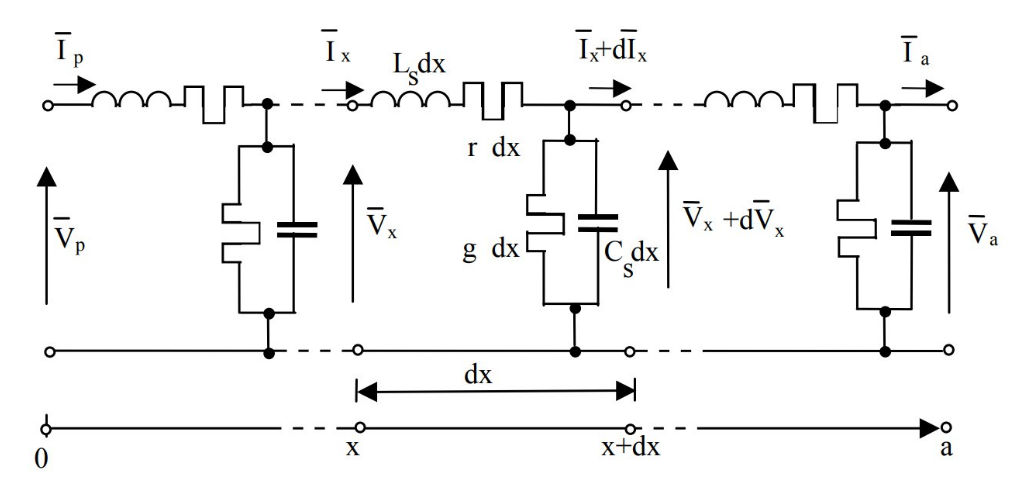
\includegraphics[width=0.6\linewidth]{immagini/regime_permanente1}
\end{figure}

Dai principi di Kirchhoff, applicati all'elemento infinitesimo, ricaviamo le seguenti relazioni:
\[\bar{V}_x - (\bar{V}_x + d\bar{V}_x) = (r \, dx + j\omega L_s \, dx) \bar{I}_x\]
\[d\bar{I}_x = -(g \, dx + j\omega C_s \, dx) (\bar{V}_x + d\bar{V}_x)\]

Trascurando gli infinitesimi del secondo ordine (ossia il termine $d\bar{V}_x \, dx$ nella seconda equazione), si ottengono le \textbf{equazioni dei telegrafisti}:
\[-\frac{d\bar{V}_x}{dx} = (r + j\omega L_s) \bar{I}_x = \bar{z}_1^l \bar{I}_x\]
\[-\frac{d\bar{I}_x}{dx} = (g + j\omega C_s) \bar{V}_x = \bar{y}_1^l \bar{V}_x\]
dove si definiscono i parametri longitudinali e trasversali per unità di lunghezza:
\begin{itemize}
    \item \textbf{Impedenza serie alla sequenza diretta ($\bar{z}_1^l$)} $\rightarrow$ definita da $\bar{z}_1^l = r + j\omega L_s$, quantifica le cadute di tensione elementari lungo la linea per unità di lunghezza.
    \item \textbf{Ammettenza derivata alla sequenza diretta ($\bar{y}_1^l$)} $\rightarrow$ definita da $\bar{y}_1^l = g + j\omega C_s$, quantifica le correnti trasversali di dispersione e capacitive per unità di lunghezza.
\end{itemize}

Derivando ulteriormente rispetto alla coordinata spaziale $x$, si ottiene:
\[\frac{d^2\bar{V}_x}{dx^2} = \bar{z}_1^l \frac{d\bar{I}_x}{dx} = \bar{z}_1^l \bar{y}_1^l \bar{V}_x = \bar{K}^2 \bar{V}_x\]
\[\frac{d^2\bar{I}_x}{dx^2} = \bar{y}_1^l \frac{d\bar{V}_x}{dx} = \bar{z}_1^l \bar{y}_1^l \bar{I}_x = \bar{K}^2 \bar{I}_x\]
avendo introdotto la costante complessa di propagazione:
\[\bar{K} = \sqrt{\bar{z}_1^l \bar{y}_1^l} = K' + jK''\]
I coefficienti caratteristici della costante di propagazione hanno il seguente significato fisico:
\begin{itemize}
    \item \textbf{Costante di attenuazione ($K'$)} $\rightarrow$ parte reale di $\bar{K}$, legata alle dissipazioni lungo la tratta; affinché la tensione in arrivo giunga con la minima attenuazione possibile, tale termine deve risultare il più piccolo possibile.
    \item \textbf{Costante di fase ($K''$)} $\rightarrow$ coefficiente della parte immaginaria di $\bar{K}$, legato allo sfasamento spaziale dell'onda viaggiante lungo la linea.
\end{itemize}
Nelle linee aeree ad altissima tensione (AT), il modulo della costante di propagazione assume tipicamente valori pari a circa $10^{-3}\text{ km}^{-1}$, discostandosi di poco dal valore della costante di fase; per esempio, in una linea a $380\text{ kV}$ con conduttori a fascio binato risulta $\bar{K} = (0{,}048 + j1{,}065) \cdot 10^{-3}\text{ km}^{-1}$.

L'integrale generale dell'equazione differenziale per la tensione presenta la forma:
\[\bar{V}_x = \bar{M} e^{\bar{K}x} + \bar{N} e^{-\bar{K}x}\]
Derivando rispetto a $x$:
\[\frac{d\bar{V}_x}{dx} = \bar{K} \bar{M} e^{\bar{K}x} - \bar{K} \bar{N} e^{-\bar{K}x}\]
e sostituendo nella prima equazione dei telegrafisti, si ricava l'espressione analitica della corrente:
\[\bar{I}_x = -\frac{1}{\bar{z}_1^l} \frac{d\bar{V}_x}{dx} = -\frac{\bar{K}}{\bar{z}_1^l} (\bar{M} e^{\bar{K}x} - \bar{N} e^{-\bar{K}x}) = -\frac{1}{\bar{Z}_0} (\bar{M} e^{\bar{K}x} - \bar{N} e^{-\bar{K}x})\]
dove si è definita l'impedenza caratteristica della linea:
\[\bar{Z}_0 = \frac{\bar{z}_1^l}{\bar{K}} = \sqrt{\frac{\bar{z}_1^l}{\bar{y}_1^l}} = \sqrt{\frac{r + j\omega L_s}{g + j\omega C_s}} = \sqrt{\frac{a(r + j\omega L_s)}{a(g + j\omega C_s)}} = \sqrt{\frac{\bar{Z}_1^l}{\bar{Y}_1^l}}\]
I parametri complessivi $\bar{Z}_1^l = a \bar{z}_1^l$ e $\bar{Y}_1^l = a \bar{y}_1^l$ rappresentano la somma delle impedenze elementari serie e delle ammettenze elementari parallelo sull'intera lunghezza $a$. Si evidenzia che per la linea a parametri distribuiti $\bar{z}_1^l \ne \bar{Z}_1^l$.

L'ordine di grandezza dell'impedenza caratteristica varia sensibilmente a seconda della tipologia costruttiva:
\begin{itemize}
    \item \textbf{Linee aeree in AT con conduttori nudi} $\rightarrow \bar{Z}_0$ assume valori dell'ordine delle centinaia di ohm (tipicamente circa $400\ \Omega$ per conduttore singolo e circa $300\ \Omega$ per fascio binato).
    \item \textbf{Linee in cavo in AT} $\rightarrow \bar{Z}_0$ assume valori nettamente inferiori, dell'ordine di $30 \div 60\ \Omega$, stante i valori notevolmente più elevati della capacità per unità di lunghezza.
\end{itemize}

Le costanti di integrazione $\bar{M}$ ed $\bar{N}$ si determinano applicando le condizioni al contorno alla sezione di partenza ($x = 0$), in cui la tensione e la corrente valgono rispettivamente $\bar{V}_p$ e $\bar{I}_p$:
\[\bar{V}_p = \bar{M} + \bar{N}\]
\[\bar{I}_p = -\frac{1}{\bar{Z}_0} (\bar{M} - \bar{N})\]
Risolvendo il sistema lineare algebrico si ottiene:
\[\bar{M} = \frac{\bar{V}_p - \bar{Z}_0 \bar{I}_p}{2}\]
\[\bar{N} = \frac{\bar{V}_p + \bar{Z}_0 \bar{I}_p}{2}\]

Sostituendo le costanti nelle relazioni di $\bar{V}_x$ e $\bar{I}_x$ e raggruppando i termini esponenziali secondo le definizioni delle funzioni iperboliche:
\[\cosh(\bar{K}x) = \frac{e^{\bar{K}x} + e^{-\bar{K}x}}{2}\]
\[\sinh(\bar{K}x) = \frac{e^{\bar{K}x} - e^{-\bar{K}x}}{2}\]
si ottengono le equazioni della linea che esprimono l'andamento della tensione e della corrente lungo la campata in funzione delle grandezze in partenza:
\[\bar{V}_x = \bar{V}_p \cosh(\bar{K}x) - \bar{Z}_0 \bar{I}_p \sinh(\bar{K}x)\]
\[\bar{I}_x = -\frac{\bar{V}_p}{\bar{Z}_0} \sinh(\bar{K}x) + \bar{I}_p \cosh(\bar{K}x)\]

\subsection{Rappresentazione come doppio bipolo}
Particolarizzando le equazioni all'ascissa di arrivo della linea ($x = a$), in cui $\bar{V}_x = \bar{V}_a$ e $\bar{I}_x = \bar{I}_a$, si ricavano:
\[\bar{V}_a = \bar{V}_p \cosh(\bar{K}a) - \bar{Z}_0 \bar{I}_p \sinh(\bar{K}a)\]
\[\bar{I}_a = -\frac{\bar{V}_p}{\bar{Z}_0} \sinh(\bar{K}a) + \bar{I}_p \cosh(\bar{K}a)\]
Invertendo la relazione per esprimere le grandezze all'origine in funzione delle grandezze al termine della tratta:
\[\bar{V}_p = \bar{V}_a \cosh(\bar{K}a) + \bar{Z}_0 \bar{I}_a \sinh(\bar{K}a)\]
\[\bar{I}_p = \frac{\bar{V}_a}{\bar{Z}_0} \sinh(\bar{K}a) + \bar{I}_a \cosh(\bar{K}a)\]

Tale formulazione coincide strutturalmente con le equazioni di trasmissione di un doppio bipolo lineare passivo simmetrico:
\[\bar{V}_p = \bar{A} \bar{V}_a + \bar{B} \bar{I}_a\]
\[\bar{I}_p = \bar{C} \bar{V}_a + \bar{D} \bar{I}_a\]
\begin{itemize}
    \item \textbf{Parametro $\bar{A}$} $\rightarrow \bar{A} = \cosh(\bar{K}a)$
    \item \textbf{Parametro $\bar{B}$} $\rightarrow \bar{B} = \bar{Z}_0 \sinh(\bar{K}a)$
    \item \textbf{Parametro $\bar{C}$} $\rightarrow \bar{C} = \frac{\sinh(\bar{K}a)}{\bar{Z}_0}$
    \item \textbf{Parametro $\bar{D}$} $\rightarrow \bar{D} = \cosh(\bar{K}a)$
\end{itemize}
Si verifica la condizione di reciprocità $\bar{A}\bar{D} - \bar{B}\bar{C} = \cosh^2(\bar{K}a) - \sinh^2(\bar{K}a) = 1$ e la condizione di simmetria longitudinale $\bar{A} = \bar{D}$.
\begin{figure}[H]
	\centering
	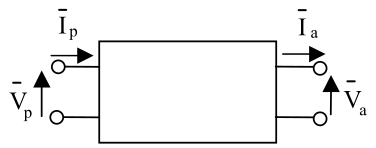
\includegraphics[width=0.4\linewidth]{immagini/regime_permanente3}
\end{figure}
Un doppio bipolo simmetrico e reciproco può essere rappresentato univocamente mediante un circuito equivalente a $\Pi$ i cui parametri $\bar{Z}^*$ e $\bar{Y}^*$ sono legati alle costanti quadripolari dalle relazioni:
\[\bar{Z}^* = \bar{B} = \bar{Z}_0 \sinh(\bar{K}a)\]
\[\bar{Y}^* = \frac{\bar{A} - 1}{\bar{B}} = \frac{\cosh(\bar{K}a) - 1}{\bar{Z}_0 \sinh(\bar{K}a)}\]
\begin{figure}[H]
	\centering
	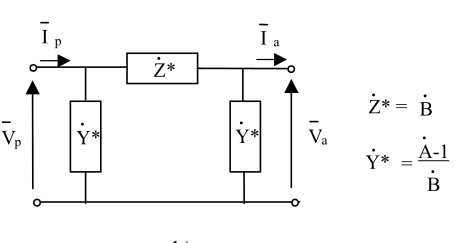
\includegraphics[width=0.5\linewidth]{immagini/regime_permanente2}
\end{figure}

\subsubsection{Modello per linea corta}
Per linee non eccessivamente lunghe (indicativamente con lunghezza $a < 400\text{ km}$), le espressioni dei parametri del circuito equivalente a $\Pi$ possono essere riscritte esplicitando il legame con l'impedenza longitudinale totale $\bar{Z}_1^l$ e l'ammettenza trasversale totale $\bar{Y}_1^l$:
\[ \bar{Z}^* = \bar{B} = \bar{Z}_0 \sinh(\bar{K}a) = \sqrt{\frac{\bar{Z}_1^l}{\bar{Y}_1^l}} \sinh\left(\sqrt{\bar{Z}_1^l \bar{Y}_1^l}\right) = \bar{Z}_1^l \frac{\sinh\left(\sqrt{\bar{Z}_1^l \bar{Y}_1^l}\right)}{\sqrt{\bar{Z}_1^l \bar{Y}_1^l}} = \bar{Z}_1^l \]
\[\bar{Y}^* = \frac{\bar{A} - 1}{\bar{B}} = \frac{\cosh\left(\sqrt{\bar{Z}_1^l \bar{Y}_1^l}\right) - 1}{\sqrt{\frac{\bar{Z}_1^l}{\bar{Y}_1^l}} \sinh\left(\sqrt{\bar{Z}_1^l \bar{Y}_1^l}\right)} = \frac{\bar{Y}_1^l}{2} \frac{\cosh\left(\sqrt{\bar{Z}_1^l \bar{Y}_1^l}\right) - 1}{\frac{\sqrt{\bar{Z}_1^l \bar{Y}_1^l}}{2} \sinh\left(\sqrt{\bar{Z}_1^l \bar{Y}_1^l}\right)}\]

Osservando che per linee corte, $|\bar{Z}_1^l \bar{Y}_1^l|<<1$, è lecito approssimare il seno iperbolico con il suo argomento e il coseno iperbolico con i primi due termini del suo sviluppo in serie di Taylor:
\[\sinh\left(\sqrt{\bar{Z}_1^l \bar{Y}_1^l}\right) \cong \sqrt{\bar{Z}_1^l \bar{Y}_1^l}\]
\[\cosh\left(\sqrt{\bar{Z}_1^l \bar{Y}_1^l}\right) \cong 1 + \frac{\bar{Z}_1^l \bar{Y}_1^l}{2}\]

Sostituendo tali sviluppi si ricavano i parametri semplificati:
\[\bar{Z}^* = \bar{Z}_1^l \frac{\sqrt{\bar{Z}_1^l \bar{Y}_1^l}}{\sqrt{\bar{Z}_1^l \bar{Y}_1^l}} = \bar{Z}_1^l = r_l + jX_l\]
\[\bar{Y}^* = \frac{\bar{Y}_1^l}{2} \frac{1 + \frac{\bar{Z}_1^l \bar{Y}_1^l}{2} - 1}{\frac{\sqrt{\bar{Z}_1^l \bar{Y}_1^l}}{2} \sqrt{\bar{Z}_1^l \bar{Y}_1^l}} = \frac{\bar{Y}_1^l}{2} = \frac{1}{2} (g_l + jB_l)\]

Il modello della linea corta ($a < 400\text{ km}$) coincide quindi con il circuito a $\Pi$ nominale, costituito dall'impedenza serie totale $\bar{Z}_1^l$ posta in ramo longitudinale e da due ammettenze trasversali pari ciascuna alla metà dell'ammettenza totale $\frac{\bar{Y}_1^l}{2}$, posizionate all'inizio e al termine della linea.
\begin{figure}[H]
	\centering
	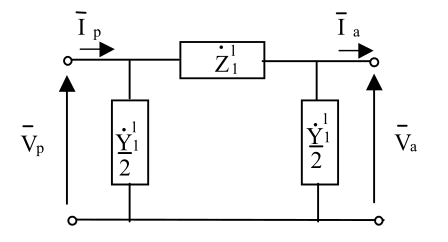
\includegraphics[width=0.4\linewidth]{immagini/regime_permanente4}
\end{figure}

\subsubsection{Modello per linea lunga}
Nel caso delle reti di distribuzione dell'energia elettrica a media tensione, le linee presentano lunghezze ridotte (tipicamente inferiori a $100\text{ km}$) e livelli di tensione non elevati. In tali condizioni le correnti capacitive e di dispersione verso terra risultano del tutto trascurabili rispetto alle correnti di carico; l'ammettenza trasversale totale $\bar{Y}_1^l$ può pertanto essere trascurata, riducendo il modello della tratta alla sola impedenza serie longitudinale $\bar{Z}_1^l$.
\begin{figure}[H]
	\centering
	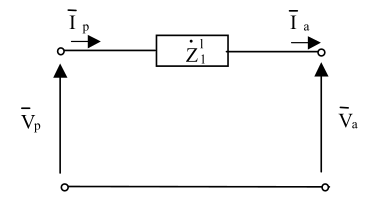
\includegraphics[width=0.4\linewidth]{immagini/regime_permanente5}
\end{figure}

\section{Modello per il trasformatore a due avvolgimenti}
Nei trasformatori di potenza trifase a due avvolgimenti, la resistenza equivalente degli avvolgimenti primario e secondario $R_{1e}$ è molto piccola rispetto alla reattanza equivalente di dispersione $X_{1e}$ ($R_{1e} \ll X_{1e}$). L'impedenza di corto circuito (o di dispersione) riportata al primario si può quindi approssimare con la sola reattanza:
\[\dot{Z}_{1e} = R_{1e} + jX_{1e} \cong jX_{1e}\]
dove:
\[Z_{1e} = \sqrt{R_{1e}^2 + X_{1e}^2} \cong X_{1e}\]

Trascurando la corrente a vuoto (magnetizzante) rispetto alla corrente nominale, il circuito monofase equivalente alla sequenza diretta riportato al primario è costituito unicamente dalla reattanza di dispersione $X_{1e}$ in serie.
\begin{figure}[H]
	\centering
	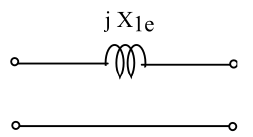
\includegraphics[width=0.3\linewidth]{immagini/regime_permanente6}
\end{figure}

Il valore della reattanza di dispersione viene determinato a partire dalla tensione di corto circuito percentuale $E_{cc\%}$, dato nominale di targa del trasformatore, mediante la relazione:
\[X_{1e} \cong Z_{1e} = \frac{E_{cc\%}}{100} \frac{E_{1n}^2}{S_n} = \frac{E_{cc\%}}{100} \frac{3 E_{1n}^2}{3 S_n}\]
avendo indicato con $E_{1n}$ la tensione nominale stellata del primario (o con $\sqrt{3}E_{1n}$ la tensione concatenata nominale $V_{1n}$) e con $S_n$ la potenza apparente nominale trifase del trasformatore. L'ordine di grandezza tipico della tensione di corto circuito percentuale per i trasformatori di potenza è compreso tra il $4\%$ e il $6\%$ ($E_{cc\%} = 4 \div 6\%$).

Nel caso in cui la potenza nominale del trasformatore non sia estremamente elevata ed è nota la potenza dissipata nella prova di corto circuito $P_{cc}$, è possibile separare il contributo resistivo da quello induttivo determinando la resistenza equivalente degli avvolgimenti:
\[R_{1e} = \frac{P_{cc}}{3 I_{1n}^2} = P_{cc} \frac{E_{1n}^2}{S_n^2}\]
e calcolando successivamente la reattanza di dispersione per differenza quadratica:
\[X_{1e} = \sqrt{Z_{1e}^2 - R_{1e}^2}\]

\section{Rappresentazione della rete a monte del punto di consegna}
\begin{figure}[H]
	\centering
	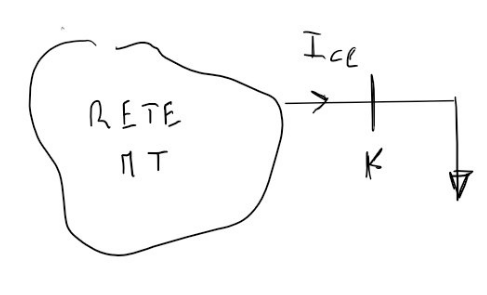
\includegraphics[width=0.45\linewidth]{immagini/regime_permanente7}
\end{figure}
Nei sistemi elettrici in media tensione (MT), la rete a monte del punto di consegna dell'energia viene modellata mediante il circuito equivalente di Thévenin, costituito da una terna di f.e.m. a vuoto alimentante l'impedenza equivalente di rete $\bar{Z}_R$.

Il distributore di energia elettrica comunica all'utente i seguenti parametri convenzionali relativi al punto di consegna:
\begin{itemize}
    \item \textbf{Corrente di corto circuito trifase ($I_{cc}$)} oppure \textbf{potenza apparente di corto circuito ($S_{cc}$)} $\rightarrow$ la corrente $I_{cc}$ rappresenta la corrente che la rete riversa nel punto di consegna (nodo $K$) qualora su di esso si verifichi un cortocircuito trifase franco a terra. La potenza apparente di corto circuito trifase vale $S_{cc} = \sqrt{3} V_{1n} I_{cc} = 3 E_{1n} I_{cc}$.
    \begin{figure}[H]
    	\centering
    	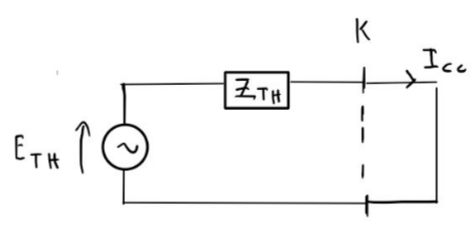
\includegraphics[width=0.45\linewidth]{immagini/regime_permanente8}
    \end{figure}
    \item \textbf{Tensione concatenata nominale ($V_{1n}$)} $\rightarrow$ corrispondente alla tensione nominale di esercizio della linea MT (con tensione stellata nominale $E_{1n} = \frac{V_{1n}}{\sqrt{3}}$).
    \begin{figure}[H]
    	\centering
    	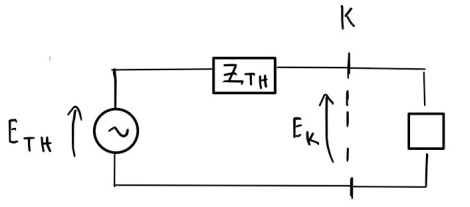
\includegraphics[width=0.45\linewidth]{immagini/regime_permanente9}
    \end{figure}
\end{itemize}

A partire da tali dati, il modulo dell'impedenza totale equivalente a monte del punto di consegna viene ricavato mediante la relazione:
\[Z_R = \frac{E_{1n}}{I_{cc}} = \frac{V_{1n}}{\sqrt{3} I_{cc}} = \frac{3 E_{1n}^2}{S_{cc}} = \frac{V_{1n}^2}{S_{cc}}\]

La scomposizione dell'impedenza di rete $\bar{Z}_R = R_R + jX_R$ nelle sue componenti resistiva e induttiva dipende dal livello di tensione e dalla tipologia delle linee:
\begin{itemize}
    \item Nelle reti con tensione nominale superiore a $35\text{ kV}$ con linee aeree prevalenti, la resistenza risulta trascurabile rispetto alla reattanza e l'impedenza di rete viene assimilata a una reattanza pura:
    \[R_R \cong 0 \implies \bar{Z}_R \cong jX_R = jZ_R\]
    \item Negli altri casi di reti MT e in assenza di dati specifici forniti dal distributore, si assume convenzionalmente il rapporto:
    \[R_R = 0{,}1 \, X_R\]
    \[X_R = 0{,}995 \, Z_R\]
\end{itemize}

\section{Modelli per il carico elettrico e il generatore sincrono}
In una rete elettrica, un carico o un generatore sincrono collegato a un nodo generico può essere schematizzato in prima approssimazione mediante un generatore ideale di corrente $\bar{I}$ uscente dal nodo (nel caso del carico) o entrante nel nodo (nel caso del generatore sincrono).
\begin{figure}[H]
	\centering
	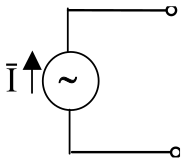
\includegraphics[width=0.2\linewidth]{immagini/regime_permanente10}
\end{figure}
La determinazione rigorosa di tali correnti risulta complessa poiché nei sistemi di potenza la corrente assorbita dalla maggior parte dei carichi dipende fortemente dalla tensione di alimentazione al nodo. Si ricorre pertanto, per i calcoli di pianificazione e di prima approssimazione, a tre modelli circuitali semplificati: a corrente costante, a impedenza costante e a potenza costante. Quando il carico si interfaccia alla rete mediante convertitori elettronici di potenza di tipo AFE (Active Front End), il comportamento del carico può essere attuato secondo una delle tre caratteristiche tramite la strategia di controllo del convertitore.

\subsubsection{Modello a corrente costante}
Nel modello a corrente costante, il carico è rappresentato da un generatore ideale di corrente il cui modulo e la cui fase rimangono invariati qualunque sia il valore della tensione al nodo.

Il valore del 	la corrente impressa viene calcolato a partire dai dati nominali di targa (potenza attiva trifase nominale $P_n$, potenza reattiva trifase nominale $Q_n$ e tensione stellata nominale $E_n$) oppure mediante calcoli di Load Flow:
\begin{figure}[H]
	\centering
	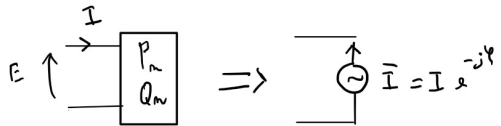
\includegraphics[width=0.5\linewidth]{immagini/regime_permanente11}
\end{figure}
\[\varphi_n = \arctan\left(\frac{Q_n}{P_n}\right)\]
\[I_n = \frac{P_n}{3 E_n \cos\varphi_n} = \frac{S_n}{3 E_n}\]

La caratteristica esterna del bipolo carico, che esprime la relazione tra la tensione ai capi del carico $E$ e la corrente assorbita $I$, assume l'equazione:
\[I = I_n = \text{cost.}\]
Tale modello, rappresentato sul piano $E\text{--}I$ da una retta verticale, non è in grado di considerare le variazioni di corrente conseguenti alle fluttuazioni della tensione di alimentazione.

\subsubsection{Modello a impedenza costante}
Nel modello a impedenza costante, assegnati i valori nominali delle potenze attiva $P_n$ e reattiva $Q_n$, il carico viene schematizzato mediante il parallelo di una conduttanza $G_n$ e di una suscettanza $B_n$, assumendo che alla tensione nominale $E_n$ l'ammettenza complessa valga:
\[\bar{Y}_n = G_n - jB_n = \frac{\bar{I}_n}{\bar{E}_n} = \frac{I_n e^{-j\varphi_n}}{E_n} = \frac{I_n}{E_n} (\cos\varphi_n - j\sin\varphi_n)\]
Moltiplicando e dividendo numeratore e denominatore per il fattore $3E_n$:
\[G_n - jB_n = \frac{3E_n I_n (\cos\varphi_n - j\sin\varphi_n)}{3E_n^2} = \frac{P_n}{3E_n^2} - j \frac{Q_n}{3E_n^2}\]
da cui l'impedenza costante equivalente:
\[\bar{Z}_n = \frac{1}{\bar{Y}_n} = \frac{3E_n^2}{P_n - jQ_n}\]

La caratteristica esterna del bipolo risponde a un modello lineare:
\[E = Z_n I = \text{cost.} \cdot I\]
Sul piano $E\text{--}I$, la caratteristica è descritta da una semiretta uscente dall'origine. Un esempio applicativo tipico è costituito dai forni elettrici a resistenza e dai riscaldatori industriali, nei quali la potenza termica dissipata varia con il quadrato della tensione di alimentazione.

\subsubsection{Modello a potenza costante}
Nel modello a potenza costante, le potenze attiva e reattiva assorbite dal carico si mantengono rigidamente fisse al variare della tensione ($P = P_n$, $Q = Q_n$). Esprimendo l'impedenza in funzione della tensione generica $E$:
\[\bar{Z} = \frac{3E^2}{P_n - jQ_n}\]
L'equazione della caratteristica esterna diviene:
\[E = Z I = \frac{3E^2}{\sqrt{P_n^2 + Q_n^2}} I = \frac{E^2}{\text{cost.}} I \implies E = \frac{\text{cost.}}{I}\]

Il legame tra tensione e corrente è descritto da un ramo di iperbole equilatera. Un esempio tipico è rappresentato da carichi motori in corrente alternata che azionano carichi meccanici a coppia resistente costante: all'instaurarsi di una repentina diminuzione della tensione di alimentazione, il motore richiede un incremento di corrente per erogare la medesima potenza meccanica all'asse.

\subsubsection{Confronto delle caratteristiche dei carichi}
\begin{figure}[H]
	\centering
	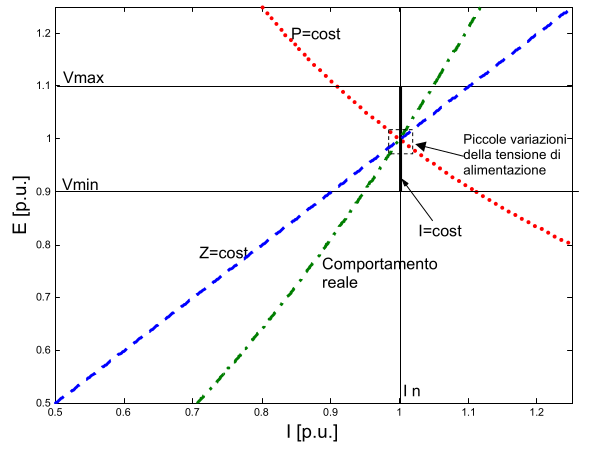
\includegraphics[width=0.7\linewidth]{immagini/regime_permanente12}
\end{figure}

Le caratteristiche dei tre modelli e la curva del carico reale presentano le seguenti peculiarità:
\begin{itemize}
    \item Le grandezze elettriche vengono normalizzate rispetto ai rispettivi valori nominali (espresse in per unit [p.u.]), fornendo un'immediata indicazione dell'ordine di grandezza.
    \item Tutte le curve si intersecano esattamente nel punto di lavoro nominale $(1{,}0\text{ p.u.}, 1{,}0\text{ p.u.})$.
    \item Per variazioni consistenti della tensione di rete al di fuori del campo di funzionamento ordinario, la corrente assorbita nel caso reale si discosta in maniera sensibile dalle previsioni: il modello a corrente costante ignora qualunque variazione, il modello a impedenza costante fornisce scostamenti differenti dalla realtà, mentre i modelli a potenza costante e reale richiedono la risoluzione di complessi sistemi algebrici non lineari.
    \item Se le oscillazioni della tensione di alimentazione rimangono contenute entro un intorno ristretto delle condizioni nominali (tipicamente $\pm 10\%$, nell'intervallo $V_{\min} \le E \le V_{\max}$), tutti i modelli approssimati convergono fornendo risultati equivalenti con un grado di accuratezza pienamente accettabile nei calcoli di rete.
\end{itemize}
